\documentclass[conference]{IEEEtran}

  \usepackage{booktabs}
  \usepackage{listing}
  \usepackage{amsmath}
  \usepackage{algorithm}
  \usepackage{array}
  \usepackage{url}
  \usepackage{cite}
  \usepackage{complexity}
\usepackage{algpseudocode}
\usepackage{graphicx}
% \usepackage{algorithm}
  \ifCLASSINFOpdf
  
  \else
  
  \fi
  
  \hyphenation{op-tical net-works semi-conduc-tor}
  
  
  \begin{document}
  
  \title{CS303 Project3: Solving Influence Maximization Problem Using the IMM Algorithm}
  
  \author{\IEEEauthorblockN{Shijie Chen}
  \IEEEauthorblockA{Department of Computer Science and Engineering\\
  Southern University of Science and Technology\\
  Shenzhen, Guangdong, China\\
  Email: 11612028@mail.sustc.edu.cn}
  }
  
  \maketitle
  
  \begin{abstract}
  The Influence Maximization Problem (IMP) has many real-world applications and is a NP-hard problem. In this project, I first developed a influence propagation model based on Linear Threshold (LT) and Independent Cascade (IC). Then, the IMM algorithm is used to solve the IMP problem. Computational experiments have shown that IMM can solve IMP problems very efficiently.
  \end{abstract}
  \IEEEpeerreviewmaketitle
  
  \section{Preliminaries}
    \subsection{Notation}
    The following notations are used in this report:
    \begin{table}[H]
        \caption{representation}
        \centering
        \begin{tabular}{cccc}
        \toprule
        Name&Variable\\
        \midrule
        The social network&$G=(V,E)$\\
        Set of edges&$E$\\
        Set of nodes&$V$\\
        Influence weight of node i to node j&$w_{ij}$\\
        Reversed reachable set&RR\\
        A node in the social network&$node$\\
        Incoming edges for a node&$incoming[]$\\
        Outgoing edges for a node&$outgoing[]$\\
    
        \bottomrule
        \end{tabular}
        \label{table:1}
        \end{table}
    \subsection{The Influence Maximization Problem}
    The influence maximization problem examines the process of the spread of influence is a social network $G$. The influence spread process is as follows:
    \begin{itemize}
        \item Initially, activate some nodes (seeds)
        \item Each node that is activated in last iteration (active nodes) stop try to activate its inactive neighbors according to a certain diffusion model.
        \item Repeat until no node is activated in an iteration.
    \end{itemize}
    Performance is given by the total number of nodes that is activated during the process.
    \subsection{Diffusion Model}
    Diffusion Model defines how influence spread in a social network. More specifically, it determines how an inactive node is activate by its active neighbors.

    \subsubsection{Linear Threshold}
    In the LT model, each node has a threshold that is assigned randomly. A node $j$ is activated if the sum of influence weight of its active neighbors $\sum\limits_{i}{w_{ij}}$ exceeds its threshold.

	\subsubsection{Independent Cascade}
    In the IC model, the process of each activated node trying to active its inactive neighbors are independent. An active node $i$ actives its inactive neighbor $j$ by probability $w_{ij}$

    \section{Methodology}
    \subsection{Data Structure}
    Data structures used in this project are $list$ and $set$.

    The social network is stored as adjacency lists in both directions to support large scale problems. Set is used to perform set operations like intersection.

    \subsection{Influence Spread Estimate (ISE)}

    As is described above, ISE is implemented by applying diffusion models on a social network $G$ with a given initial seed set $S$. 

    Note that we just need to look at neighbors of newly activated nodes to find inactive nodes that may be activated in the next iteration. In this way, we can reduce redundant computation.

    Since influence spread is a stochastic process, we take the average of 10,000 runs as the final result.

    \begin{algorithm}[H]
        \begin{algorithmic}[1]
            \Function{IC}{outgoing,seedSet}
            \State $activatedNodes \gets seedSet$
            \State $activity \gets seedSet$
            \While {$activity \neq \emptyset$}
                \State $newSet \gets \emptyset$
                \For {$i\in activity$}
                    \For{$j \in outgoing[node]$}
                        \If {$j \; is \; not \; activated$}
                            \State $prob \gets random(0,1)$
                            \If{$prob \leq w_{ij}$}
                                \State $activatedNodes.add(j)$
                                \State $newSet.add(j)$
                            \EndIf
                        \EndIf
                    \EndFor
                \EndFor
                \State $activity \gets newSet$
            \EndWhile


            \Return $len(activatedNodes)$
            \EndFunction
        \end{algorithmic}
        \caption{ISE IC}
    \end{algorithm}

    \begin{algorithm}[H]
        \begin{algorithmic}[1]
        \Function{LT}{incoming, outgoing,seedSet}
        \State $activatedNodes \gets seedSet$
        \State $activity \gets seedSet$
        \State $randomly\; assign\; threshold\; to\; each\; node$
        \While {$activity \neq \emptyset$}
            \State $newSet \gets \emptyset$
            \For {$node\in activity$}
                \For{$ j\in outgoing[node]$}
                    
                    \If {$neighbor \; is \; not \; activated$}
                        \State $influence \gets 0$
                        \For {$ i \in incoming[j])$}
                            \If {$i \; is\;activated$}
                            \State $influence \gets influence + w_{ij}$
                            \EndIf
                        \EndFor

                        \If{$influence \leq j.threshold$}
                            \State $activatedNodes.add(j)$
                            \State $newSet.add(j)$
                        \EndIf
                    \EndIf
                \EndFor
            \EndFor
            \State $activity \gets newSet$
        \EndWhile


        \Return $len(activatedNodes)$
        \EndFunction
        \end{algorithmic}
        \caption{ISE LT}
    \end{algorithm}

    \subsection{Influence Maximization Problem (IMP)}
    There are many algorithms that can solve IMP. In this project, I implemented an algorithm that is based on IMM \cite{Tang:2015:IMN:2723372.2723734} and introduced parallelism to accelerate the algorithm. The IMM algorithm provides a $(1-1/e-\varepsilon)$-approximate solution to IMP and performs well in large scale problems.
    The algorithm is composed of two phases:

    \begin{itemize}
        \item \textbf{Sampling}
        This step generates random reversed reachable sets and put them together as a set $\mathcal{R}$ until a stopping criteria is met.

        
        
        To generate a RR set, we start from a randomly chosen node v, apply influence spread in a reversed direction and return the activated nodes. Which is to say, active nodes will try to activate inactive neighbors in $incoming[node]$ according to IC or LT model. The process is almost the identical to ISE, so details are omitted in this report.
        \begin{algorithm}[H]
            \begin{algorithmic}[1]
            \Function{genRR}{$v$}
            \State $RR \gets reversedISE(v)$

            \Return $RR$
            \EndFunction
            \end{algorithmic}
            \caption{genRR}
        \end{algorithm}

        
        \begin{algorithm}[H]
            \begin{algorithmic}[1]
            \Function{LT}{$G,k,\varepsilon,l$}
            \State $\mathcal{R} \gets \emptyset$
            \State $LB = 1$
            \State $\varepsilon^{\prime} \gets \sqrt{2} \cdot \varepsilon$
            \For {$i \gets 1 \; to \; \log_{2} n - 1$}
                \State $x \gets n/2^i$
                \State $\theta_{i} \gets \lambda^{\prime}$
                \While {$len(\mathcal{R}) \leq \theta_i$}
                \State $ randomly\;select\;a\;node\;v\;from\;G$
                \State $RR \gets \Call{genRR}{$v$}$
                \State $\mathcal{R}.append(RR)$
                \EndWhile
                \State $S_i \gets \Call{nodeSelection}{\mathcal{R}}$
                \If {$n \cdot F_{\mathcal{R}}\geq (S_i)/(1+\varepsilon^{\prime})$}
                    \State $LB \gets n\cdot F_{\mathcal{R}}(S_i)/(1+\varepsilon^{\prime})$
                    \State \textbf{break}
                \EndIf
            \EndFor
            \State $\theta \gets \lambda^{*}/LB$
            \While {$len(\mathcal{R}) \leq \theta$}
            \State $ randomly\;select\;a\;node\;v\;from\;G$
            \State $RR \gets \Call{genRR}{$v$}$
            \State $\mathcal{R}.append(RR)$
            \EndWhile 


            \Return $\mathcal{R}$
            \EndFunction
            \end{algorithmic}
            \caption{Sampling}
        \end{algorithm}

        \item \textbf{Node Selection}
        This step selects $k$ solutions from $\mathcal{R}$ to form a size-$k$ solution set $S_{k}^*$ that covers the most RR sets. $S_{k}^*$ is returned as the final result. $F_{\mathcal{R}}(S)$ returns the number of RR sets in $\mathcal{R}$ that overlaps S. 
        
        $$F_{\mathcal{R}}(S) = \vert \{ RR|RR \cap S \neq \emptyset, RR \in \mathcal{R}\} \vert $$
        This step can be optimized to reduce computation of $F_{\mathcal{R}}(S)$. We can keep track of the number of sets a node $v$ can activate if it is added to $S_k^*$ with a list $hit[]$. Each time we take the $v$ with the largest $hit[v]$, insert $v$ to $S_k^*$ and update $hit[]$.
        \begin{algorithm}[H]
            \begin{algorithmic}[1]
            \Function{NodeSelection}{$\mathcal{R},k$}
            \State $S_k^{*} \gets \emptyset$
            \For {$i \gets 1\;to\; k$}
                \State $v \gets \underset{v}{\mathrm{argmax}} \{F_{\mathcal{R}}(S_k^* \cup v)-F_{\mathcal{R}}(S_k^*)\}$
                \State $S_k^* \gets S_k^* \cup v$
            \EndFor
            


            \Return $S_k^*$
            \EndFunction
            \end{algorithmic}
            \caption{NodeSelection}
        \end{algorithm}
    \end{itemize}

    The IMM algorithm put together the above two phases.

    \begin{algorithm}[H]
        \begin{algorithmic}[1]
        \Function{IMM}{$G,k,\varepsilon,l$}
        \State $l \gets l \cdot (1+\log_n 2)$
        \State $\mathcal{R} \gets \Call{Sampling}{G,k,\varepsilon,l}$
        \State $S_k^* \gets \Call{NodeSelection}{\mathcal{R},k}$

        \Return $S_k^*$
        \EndFunction
        \end{algorithmic}
        \caption{IMM}
    \end{algorithm}
\subsection{Parameters}
There are many parameters in the IMM algorithms. The values are chosen so as to guarantee a $(1-1/e-\varepsilon)$-approximate result. $l$ and $\varepsilon$ are two external parameters. For IMM in this report, I used $l = 1$ and $\varepsilon = 0.1$.

Parameters are computed as follows:
\begin{equation}
\alpha = \sqrt{l \log n+\log 2} 
\end{equation}
\begin{equation}
\beta = \sqrt{(1-1/e)\cdot (\log {n\choose k}+l\log n + \log 2)}
\end{equation}
\begin{equation}
\lambda^* = 2n((1-1/e)\cdot \alpha + \beta)^2\cdot\varepsilon^{-2}
\end{equation}    
\begin{equation}
\lambda = (8+2\varepsilon)n\cdot(l\log n+\log{n\choose k}+\log2)
\end{equation}

IMM is designed to finish in $O((k+l)(n+m)\log n/\varepsilon^2)$ time and returns a $(1-1/e-\varepsilon)$-approximate solution with at least $1-1/n^l$ probability under triggering model(In this report, IC and LT)\cite{Kempe:2003:MSI:956750.956769}. For IMM, we set $l = 1$.

$\varepsilon \in (0,1)$ is a parameter that can be set by the user to control accuracy. A lower $\varepsilon$ value will increase accuracy but will increase computation time dramatically. I used $\varepsilon = 0.1 $ to balance accuracy and computation time.

\section {Parallel Implementation}
In this project, I used parallel programming in ISE and Sampling phase of IMM.

In ISE, the process of computing average score is conducted in parallel.

In IMM, the process of generating RR sets is conducted in parallel.

Unfortunately, experiments show that most of the computation time in IMM is used by $nodeSelection$ method.

\section{Validation}
\subsection{Environment}     
\begin{itemize}
    \item OS: windows 10
    \item RAM: 16G
    \item CPU: Intel Core i7 8700k @ 3.7GHz
    \item Python: 3.7.1
\end{itemize}
The parallel part of the program uses 8 processes.
\subsection{ISE}
ISE is run 10000 times on the $network$ data set with two seed sets and the result is the average value.
\begin{table}[H]
    \caption{representation}
    \centering
    \begin{tabular}{cccc}
    \toprule
    Benchmark&Diffusion Model&Time(s)&Result\\
    \midrule
    network-seeds&IC&1.108&5.037\\
    network-seeds&LT&1.101&5.053\\
    network-seeds2&IC&1.110&30.423\\
    network-seeds2&LT&1.239&37.145\\
    \bottomrule
    \end{tabular}
    \label{table:1}
    \end{table}

\subsection{IMP}
IMP is run on the $network$ and $NetHeap$ data sets.

\begin{table}[H]
    \caption{representation}
    \centering
    \begin{tabular}{ccccc}
    \toprule
    Benchmark&Diffusion Model&$k$&Time(s)&Result\\
    \midrule
    network&IC&5&0.387&30.636\\
    network&LT&5&0.229&37.653\\
    NetHeap&IC&5&6.954&323.585\\
    NetHeap&LT&5&6.312&392.521\\
    NetHeap&IC&50&9.766&1296.445\\
    NetHeap&LT&50&8.915&1698.013\\
    
    \bottomrule
    \end{tabular}
    \label{table:1}
    \end{table}

    \section{Discussion}

    Computational experiments show that my implementation of ISE can estimate influence spread process quite accurately and my implementation of IMP can obtain good result in an acceptable time.

    While my IMP implementation perform well under LT model, performance is not so good under IC model compared to others' algorithms. 

    Moreover, experiments also show that most of the computation time of my implementation of IMP is consumed by node selection, as is shown in 
    \begin{figure}[H]
    \centering
    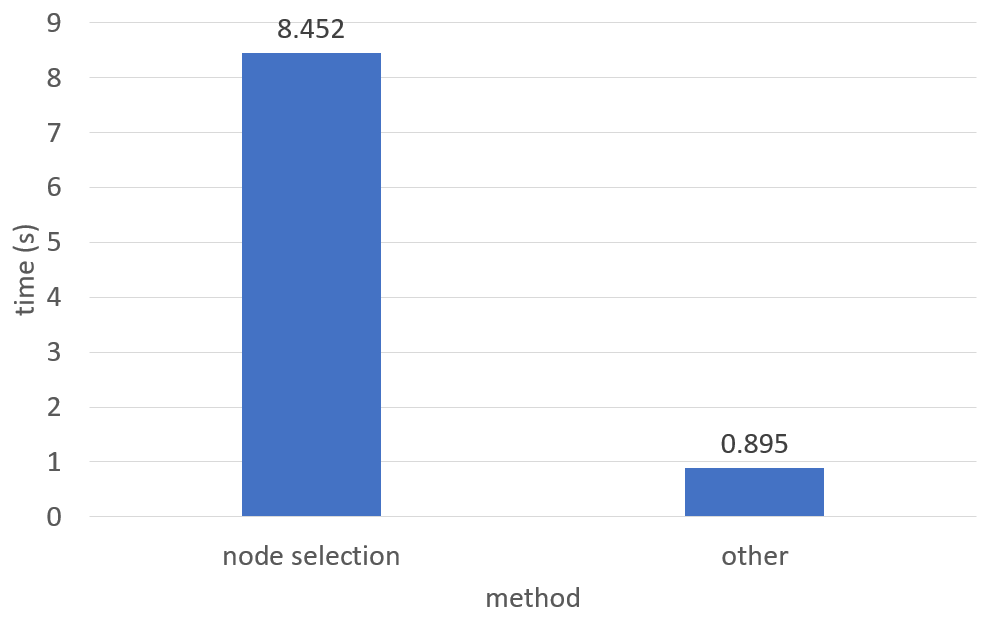
\includegraphics[width=0.4\textwidth]{time.png}
    \caption{Running time of IMM under NetHeap, $k$ = 50, IC}
    \label{fig1}
    \end{figure}
    
    A better implementation of node selection may be used and hopefully it can make use of parallelism.

\section{Conclusion}

In this project, I implemented ISE with IC and LT model and IMP using IMM algorithm. The performance is generally good. Some improvement can be made to improve the efficiency of implementation.
\section*{Acknowledgment}

The authors would like to thank the TAs for their hint in the Lab and maintaining a online runtime platform. 


\bibliographystyle{ieeetr}
\bibliography{ref}



% that's all folks
\end{document}


  